\chapter{Specyfikacja wewnętrzna}\label{Chapter_SpecyfikacjaWewnetrzna}

  \section{Wykorzystane technologie}\label{Section_Technologie}

    \subsection{C++}\label{Subsection_Cpp}
      Proces tworzenia oprogramowania przeszedł diametralne zmiany w~ostatnim dziesięcioleciu. Sformułowanie w~roku~2001 tzw. \textit{manifestu metodyk zwinnych} poruszyło klasyczny model tworzenia oprogramowania. Wspomniana ewolucja dotknęła także języki programowania. W~obecnych czasach zdecydowanie większą popularnością cieszą się języki dynamiczne (w~większości przypadków \textit{interpretowane} takie jak \textit{Ruby}, \textit{Python} lub \textit{JavaScript}), lub kompilowane do kodu pośredniego, specyficznego dla danej platformy uruchomieniowej (przykładem są języki \textit{Java} oraz \textit{C\#}).

      Przymiotniki \textit{lekki} i~\textit{zwinny}, będące podstawą wspomnianego manifestu są przede wszystkim fundamentem języków dynamicznych, ale również tych ewoluujących bardzo szybko. Język \textit{C++} zdecydowanie nie należy do tej grupy. To język statycznie typowany, o~dużej dojrzałości, czerpiący pełnymi garściami z~równie znanego poprzednika jakim jest język \textit{C}. Niestety ewoluuje on bardzo wolno (co związane jest z~dojrzałością oraz próbami zachowania kompatybilności wstecznej z~poprzednikiem), przez co stracił popularność w~obecnych czasach.

      Nadal jednak to języki kompilowane do kodu maszynowego, pod konkretną architekturę i~model procesora są w~wielu zastosowaniach niezastąpione. Tworzenie niskopoziomowego oprogramowania, tworzenie sterowników urządzeń czy aplikacji o~maksymalnych wymaganiach określonych w~zakresie wydajności to obszary gdzie język \textit{C++} i~jego poprzednicy są nadal najpopularniejszym i~najefektywniejszym wyborem. Przetwarzanie obrazów i~algorytmy wizyjne zdecydowanie należą do ostatniej grupy, przez co wszystkie najpopularniejsze biblioteki i~znaczące algorytmy są implementowane właśnie w~tych językach.

      \subsubsection{Standard ISO C++ z~roku~2003}
      Obowiązującym standardem języka \textit{C++} jest standard \textit{ISO/IEC 14882:1998} (\textit{Standard for the C++ Programming Language}) z drobnymi poprawkami zatwierdzonymi w~2003~r. (\textit{ISO/IEC 14882:2003}). W~2009 roku ogłoszono nowy standard (tzw.~\textit{C++0x}), który zaczął obowiązywać od 12 sierpnia 2011 roku, lecz wciąż oczekuje na opublikowanie (\textit{ISO/IEC 14882:2011}).

      Ostatnia wersja, wciąż oczekująca na publikację, wprowadza wiele nowości zdecydowanie ułatwiających tworzenie oprogramowania. Ujednolicono wiele koncepcji i~co najważniejsze znacznie poszerzono bibliotekę standardową co ułatwi pracę programistów i~zredukuje ilość zewnętrznych zależności niezbędnych do kompilacji. Duży udział w~rozszerzeniu biblioteki standardowej miała społeczność i~autorzy poszczególnych modułów biblioteki \textit{boost}, która jest najważniejszą i~najpopularniejszą biblioteką (wyłączając bibliotekę standardową) w~środowisku programistów \textit{C++}.

      W~pracy wykorzystano stabilną i~dojrzałą wersję standardu z~roku 2003. Istnieje wiele publikacji (najpopularniejszymi są \cite{EffectiveCpp}, \cite{MoreEffectiveCpp}, \cite{EffectiveStl} oraz \cite{Alexandrescu}) oraz materiałów na temat (biblioteka \textit{MSDN} oraz dokumentacja biblioteki \textit{STL}), jak efektywnie korzystać z~dostępnej funkcjonalności i~przede wszystkim jak unikać \textit{pułapek} oraz w~jaki sposób efektywnie korzystać z~mnogości dostępnych paradygmatów i~rozwiązań udostępnionych w~specyfikacji języka.

      \subsubsection{Programowanie Obiektowe}
      Język \textit{C++} jest językiem wieloparadygmatowym, jednak dominującym paradygmatem tworzenia oprogramowania w~języku \textit{C++} jest tzw. \textit{programowanie obiektowe} (ang. \textit{Object Oriented Programming} w~skrócie \textit{OOP}). Wspomniany wyżej standard z~2003~roku posiada największe wsparcie właśnie dla tego paradygmatu, dodatkowo w~czasach największej popularności tego języka to właśnie programowanie obiektowe było najpopularniejsze.

      Koncepcja programowania obiektowego sięga języka \textit{Simula 67}, następnie dopracowano wszystkie koncepty w~języku \textit{Smalltalk}. Sam język \textit{C++}, którego pierwsza koncepcja pojawiła się w~1979 roku, intensywnie korzysta z~elementów programowania obiektowego wprowadzonych właśnie w~języku \textit{Simula}, jak również z~języków takich jak \textit{Algol}, \textit{Ada} czy \textit{ML} \cite{CppStroustrup}.

      Programowanie obiektowe opiera się na czterech filarach, którymi są:
      \begin{itemize}
        \item \textbf{Abstrakcja} - Każdy obiekt w~systemie służy jako model abstrakcyjnego \textit{wykonawcy}, który może wykonywać pracę, opisywać i~zmieniać swój stan oraz komunikować się z~innymi obiektami w~systemie bez ujawniania, w~jaki sposób zaimplementowano dane cechy. Procesy, funkcje lub metody mogą być również abstrahowane, a~kiedy tak się dzieje, konieczne są rozmaite techniki rozszerzania abstrakcji.

        \item \textbf{Hermetyzacja} - Potocznie: ukrywanie implementacji, dokładnie: \textit{enkapsulacja}. Zapewnia, że obiekt nie może zmieniać stanu wewnętrznego innych obiektów w~nieoczekiwany sposób. Tylko własne metody obiektu są uprawnione do zmiany jego stanu. Każdy typ obiektu prezentuje innym obiektom swój interfejs, który określa dopuszczalne metody współpracy. Pewne języki~osłabiają to założenie, dopuszczając pewien poziom bezpośredniego (kontrolowanego) dostępu do stanu wewnętrznego obiektu. Ograniczają w~ten sposób poziom abstrakcji. Przykładowo w~niektórych kompilatorach języka \textit{C++} istnieje możliwość tymczasowego wyłączenia mechanizmu enkapsulacji; otwiera to dostęp do wszystkich pól i~metod prywatnych, ułatwiając programistom pracę nad pośrednimi etapami tworzenia kodu i~znajdowaniem błędów.

        \item \textbf{Polimorfizm} - Referencje i~kolekcje obiektów mogą dotyczyć obiektów różnego typu, a~wywołanie metody dla referencji spowoduje zachowanie odpowiednie dla pełnego typu obiektu wywoływanego. Jeśli dzieje się to w~czasie działania programu, to nazywa się to \textit{późnym wiązaniem} lub \textit{wiązaniem dynamicznym}. Niektóre języki udostępniają bardziej statyczne (w trakcie kompilacji) rozwiązania polimorfizmu – na przykład szablony i~przeciążanie operatorów w~\textit{C++} \cite{CppStroustrup}.

        \item \textbf{Dziedziczenie} - Porządkuje i~wspomaga polimorfizm, i~enkapsulację dzięki umożliwieniu definiowania, i~tworzenia specjalizowanych obiektów na podstawie bardziej ogólnych. Dla obiektów specjalizowanych nie trzeba przedefiniowywać całej funkcjonalności, lecz tylko tę, której nie ma obiekt ogólniejszy. W typowym przypadku powstają grupy obiektów zwane \textit{klasami}, oraz grupy klas zwane \textit{hierarchiami dziedziczenia}. Odzwierciedlają one wspólne cechy obiektów.
      \end{itemize}

      \subsubsection{Zastosowanie programowania obiektowego w~wizji komputerowej}
      \textit{Jakość} jest subiektywnym i~niemierzalnym współczynnikiem podstawowego budulca aplikacji, jakim jest kod źródłowy. Niezmiernie ważnym jest, aby podczas procesu tworzenia oprogramowania, korzystać ze~zbioru sprawdzonych praktyk i~rozwiązań oraz pilnować spójności tworzonego produktu końcowego. Równie ważnym elementem jest dobór paradygmatu, w~jakim tworzona jest implementacja, do możliwości głównego narzędzia jakim jest język programowania i~wykorzystane biblioteki.

      Implementacja zaprezentowana w~pracy oparta jest na języku \textit{C++} oraz bibliotece \textit{OpenCV}, dlatego zastosowanym paradygmatem jest opisywane \textit{programowanie obiektowe}. Zgodnie z~pierwszym z~podstawowych filarów programowania obiektowego - \textit{Abstrakcją} - każda implementacja określonego algorytmu śledzenia punktów charakterystycznych jest wyabstrahowanym wykonawcą. Wszystkie implementacje korzystają z~wspólnej abstrakcyjnej klasy bazowej, natomiast detale i~sposób interakcji z~biblioteką oraz sekwencją obrazów został ukryty wewnątrz konkretnych przypadków.

      W~tym przypadku wykorzystanie abstrakcyjnej klasy bazowej to użycie \textit{Strategii}, jednego z~\textit{czynnościowych wzorców projektowych}. Zgodnie z~definicją zamieszczoną w~\cite{PatternsGoF} ten wzorzec projektowy definiuje rodzinę wymiennych algorytmów i~kapsułkuje je w postaci klas. Dzięki temu możliwe jest wymienne stosowanie każdego z~nich w~trakcie działania aplikacji niezależnie od korzystających z~nich klientów.

      Kolejną ważna abstrakcją z~punktu widzenia algorytmów przetwarzania sekwencji wideo jest klasa strumienia o~nazwie \textit{VideoStream}, która zostanie dokładnie opisana w~rozdziale \ref{Section_ImplementationDetails}. Tworzy ona abstrakcję sekwencji klatek, wraz z~możliwością wykorzystania jednego lub wielu algorytmów zgodnych z~wspomnianym wzorcem \textit{Strategii}. Dodatkowo klasa ta umożliwia otoczenie wywołań metod przetwarzających pojedynczą klatkę i~cały strumień wideo, w~celu pomiaru czasu wykonania lub ilości zużytej pamięci.

    \subsection{STL}\label{Subsection_STL}

      \subsubsection{Opis biblioteki}
      Główną częścią biblioteki standardowej języka \textit{C++} jest \textit{standardowa biblioteka szablonów} (ang. \textit{Standard Template Library}). Zawiera ona algorytmy, pojemniki, iteratory i~inne konstrukcje w~formie szablonów, przetestowane oraz gotowe do użycia przy tworzeniu oprogramowania. Głównym architektem w~początkowym stadium rozwoju tej biblioteki był \textit{Alexander Stepanov} i~na początku powstawała ona jako niezależna biblioteka rozwijana przez firmę \textit{Hewlett Packard}. Z~czasem większość przyjętych tam form wyewoluowała do formy biblioteki standardowej (w~standardzie z~roku 2003 znajduje się praktycznie większość konceptów przeniesionych ze wspomnianego pierwowzoru). Dominującym paradygmatem wykorzystywanym w~\textit{STL} jest programowanie generyczne i~dzięki temu jej składniki dobrze współpracują, z~typami wbudowanymi w~język, samą bibliotekę jak i~tymi zdefiniowanymi przez użytkownika \cite{StlJosuttis}.

      \subsubsection{Szablony}
      Fundamentem biblioteki \textit{STL} i~paradygmatu programowania generycznego (\textit{uogólnionego}) jest funkcjonalność \textit{Szablonów} dostarczana przez język \textit{C++}. Jest to możliwość tworzenia kodu programu bez wcześniejszej znajomości typów danych, na których ten będzie operował. Ten typ programowania umożliwia językom statycznie typowanym na polimorfizm typów.

      Wykorzystanie szablonów w~programach pozwala skupić się bardziej na algorytmach niż na danych jakie są przetwarzane. Użycie szablonów pozwala zredukować ilość nadmiarowego kodu ponieważ jedną funkcjonalność można zaprogramować dla wielu typów danych. Następnie kompilator w konkretnym przypadku precyzuje typ i~odpowiednio dostosowuje np. wywołania funkcji. Podczas kompilacji następuje tak zwana konkretyzacja szablonu (ang. \textit{template instantiation}), podczas której kompilator na podstawie typów danych przekazanych wzorcowi generuje kod właściwy do obsługi danego typu.

      \subsubsection{Algorytmy}
      Jedną z~podstawowych koncepcji zwartych w~\textit{STL} jest koncepcja algorytmu działającego w~oderwaniu od implementacji pojemnika. Do mediacji między pojemnikiem a~faktyczną implementacją wykorzystywany jest wzorzec \textit{Iterator} (szczegóły można znaleźć w~\cite{PatternsGoF}). Każdy z~kontenerów implementuje określony zestaw \textit{iteratorów}, które umożliwiają poruszanie się po kolejnych elementach zebranych w~kolekcji.

      Odstąpienie od powiązania abstrakcyjnego algorytmu z~implementacją pojemnika wiąże się z~wykorzystaniem \textit{idiomów}, które zostaną szerzej opisane w~jednej z~poniższych sekcji.

      Dodatkowo niektóre kolekcje posiadają własne implementacje algorytmów, przykładem może być algorytm sortowania dla kontenera list dwukierunkowych \textit{list}. W~takim przypadku zaleceniem jest wykorzystanie metody zaimplementowanej w~kontenerze, ponieważ w~większości przypadków będzie ona zoptymalizowana (dzięki wiedzy o~wewnętrznej strukturze i~implementacji danej struktury) \cite{EffectiveStl}. Wydajniejsze rozwiązanie jest obarczone w~tym przypadku powiązaniem między algorytmem a~konkretną implementacją kolekcji.

      \subsubsection{Funktory}
      Kolejnym bardzo ważnym konceptem zastosowanym w~bibliotece \textit{STL} jest abstrakcja \textit{Funktora} (ang. Functors) lub inaczej \textit{Obiektu Funkcyjnego}. Jest to klasa z~przeładowanym operatorem wywołania metody (\textit{operator()}). Możliwe jest parametryzowanie stworzonego obiektu za pomocą konstruktora oraz przechowywanie wewnętrznego stanu \textit{funktora} wewnątrz pól klasy. Ponieważ \textit{obiekt funkcyjny} i~wskaźniki na funkcje mogą być wywołane za pomocą tej samej składni mogą być stosowane zamiennie właśnie jako argumenty szablonów.

      Najpopularniejszą koncepcją związaną z~\textit{funktorami} jest \textit{Predykat}. Jest to koncept zaczerpnięty z~matematyki. Jest to definicja pewnej funkcji logicznej (\textit{boolowskiej}) o~dowolnej dziedzinie i~przeciwdziedzinie będącej zbiorem wartości logicznych (\textit{prawda}, \textit{fałsz}). W~przypadku \textit{STL} wewnętrzna implementacja funktora na podstawie parametrów wejściowych podejmuje decyzje o~przypisaniu określonej wartości logicznej związanej z~przekazanymi argumentami.

      \subsubsection{Idiomy}\label{Idioms}
      Bardzo ważnym elementem podczas wykorzystywania \textit{standardowej biblioteki szablonów} jest trzymanie się określonych warunków wymaganych od typów zdefiniowanych przez użytkownika, ale także zbioru wypracowanych technik zwanych \textit{idiomami}. Pomocnym źródłem jest pozycja \cite{EffectiveStl} ilustrująca wiele przykładów wspomnianych idiomów oraz prezentująca potencjalne pułapki i~sytuacje, których użytkownicy biblioteki powinni unikać. Poniżej zamieszczony został przykład jednego z~idiomów zwanego \textit{erase-remove}, służącego do zwolnienia miejsca w~pojemniku zajmowanego przez elementy oznaczone jako usunięte (ponieważ algorytm \textit{remove} sam w~sobie nie usuwa elementów zgromadzonych w~kontenerze, jedynie przenosi je na koniec i~oznacza jako usunięte, faktyczne usunięcie może wykonać dopiero metoda \textit{erase} zaimplementowana w~określonym pojemniku).

      \begin{sample}[ht]
        \begin{verbatim}
std::vector<int> v = { 0, 1, 2, 3, 4, 5, 6 };

// Usunięcie elementów o wartości 5.
v.erase(std::remove(v.begin(), v.end(), 5), v.end());
        \end{verbatim}
        \caption{Idiom erase-remove wykorzystywany w~bibliotece STL}
        \label{EraseRemoveIdiom}
      \end{sample}

    \subsection{OpenCV}\label{Subsection_OpenCV}

      \subsubsection{Opis biblioteki}
      \textit{OpenCV} jest jedną z~najpopularniejszych bibliotek (jeśli nie najpopularniejszą) związanych z~wizją komputerową. Zawiera funkcje wykorzystywane do obróbki obrazu, sekwencji wideo jak również i~struktury służące do uczenia maszynowego lub funkcje pomocnicze dla graficznego interfejsu użytkownika.

      Oparta jest na otwartej licencji \textit{BSD} i~jej rozwój został zapoczątkowany została przez firmę \textit{Intel} w~1999 roku. Jest ona napisana w~języku \textit{C++} i~głównym interfejs programistyczny jest dostosowany właśnie do tego języka, niemniej starsze implementacje przygotowane w~języku \textit{C} są ciągle dostępne i~istnieje możliwość ich wykorzystania.

      \textit{OpenCV} jest wieloplatformową biblioteką, w~pełni współpracującą z~systemami operacyjnymi \textit{Mac OS X}, \textit{Microsoft Windows} i~\textit{Linux}. W~momencie tworzenia pracy wykorzystywana była aktualnie dostępna wersja o~numerze \textit{2.4.3}. Popularność tej biblioteki przyniosła, z~pomocą społeczności, interfejsy programistyczne do praktycznie każdego popularnego języka programowania. Warto nadmienić, że obecnie wszelkiego rodzaju nowe funkcjonalności implementowane są w~języku \textit{C++}, włączając w~to wsparcie dla platform \textit{CUDA} i~podobnych.

      Dokumentacja dostępna na oficjalnej stronie internetowej jest obszerna i~wraz z~zamieszczonymi przykładami tworzy kompletny poradnik. Dodatkowo istnieje kilka pozycji bibliograficznych na rynkach zagranicznych, które zostały wykorzystane przy tworzeniu pracy \cite{LearningOpenCV}, \cite{OpenCVCookbook}.

      \subsubsection{Podstawowe koncepcje wykorzystywane przy pracy z~OpenCV}
      W~kontekście omawianej pracy biblioteka \textit{OpenCV} udostępnia wiele konceptów, które ułatwiają pracę i~pozwalają skupić się na faktycznej implementacji algorytmów. Intensywnie wykorzystywane są następujące elementy:
      \begin{itemize}
        \item Wczytywanie i~zapis różnorakich formatów sekwencji wideo.
        \item Podstawowe operacje i~filtry zdefiniowane jako pojęcia wizji komputerowej.
        \item Metody pomocnicze wspomagające implementację algorytmów śledzenia punktów charakterystycznych.
        \item Struktury ułatwiające realizację algorytmów opartych o~uczenie maszynowe.
      \end{itemize}

      Oprócz elementów zawartych w~bibliotece \textit{OpenCV} niezbędne było również wprowadzenie nowych abstrakcji ułatwiających operowanie na sekwencjach wideo (które zostały pobieżnie omówione w~sekcji \textit{Zastosowanie programowania obiektowego w~wizji komputerowej} i~zostaną omówione dokładniej w~podrozdziale \ref{Section_ImplementationDetails}).

    \subsection{Narzędzia pomocnicze}\label{Subsection_PomocniczeTechnologie}

      \subsubsection{Biblioteka d3.js}
      \textit{D3} to środowisko do obliczeń statystycznych oraz wizualizacji wyników (za pomocą przeglądarki internetowej, w~formacie wektorowym SVG) napisana w~języku JavaScript. Znajduje on zastosowanie w~każdej dziedzinie nauki wymagającej analizy statystycznej i~prezentacji wyników w~postaci różnego rodzaju wykresów. Została ona szczegółowo opisana w~książce \cite{D3Book}.

      W~pracy zostały wykorzystane skrypty opierające się o~pakiety analizy statystycznej oraz prezentacji wyników pomiarów poszczególnych implementacji i~algorytmów. Poniżej zaprezentowano przykładowy skrypt, pozostałe wykresy oraz analiza statystyczna znajdują się w~rozdziale \ref{Chapter_AnalizaRezultatow}.

      \begin{sample}[ht]
        \begin{verbatim}
(function(d3, nv) {
  var chart = nv.models.lineChart();

  chart.xAxis
    .axisLabel(config.xLabel)
    .tickFormat(d3.format(config.xFormat || ",r"));

  chart.yAxis
    .axisLabel(config.yLabel)
    .tickFormat(d3.format(config.yFormat || ".02f"));

  d3.select("#charts")
    .insert("section", ":first-child")
      .append("svg")
        .datum(config.extractor(results))
          .call(chart);

  d3.select("#charts")
    .insert("h2", ":first-child")
    .text(config.name);

  nv.utils.windowResize(chart.update);

} (window.d3, window.nv));
        \end{verbatim}
        \caption{Skrypt przygotowujący wykres liniowy za pomocą biblioteki d3.js}
        \label{ChartForRunningTimePerAlgorithm}
      \end{sample}

      \subsubsection{HTML5, CSS3 i~warstwa pośrednia oparta o~NodeJS}\label{Subsection_NodeJS}
      Ważnym elementem jest selekcja punktów charakterystycznych w~zarejestrowanych sekwencjach wideo. W~tym celu przygotowane zostało proste narzędzie oparte w~całości na technologiach internetowych. Interfejs użytkownika został zaprojektowany i~przygotowany za pomocą \textit{HTML5} oraz \textit{CSS3}.

      Za warstwę pośrednią (spajającą interfejs użytkownika oraz implementacje algorytmów przygotowane w~języku \textit{C++}) odpowiada środowisko uruchomieniowe \textit{NodeJS}. Jest to środowisko uruchomieniowe oprogramowywane za pomocą języka \textit{JavaScript}, które wraz z~biblioteką \textit{express} umożliwia udostępnienie statycznych zasobów (takich jak skrypty, kaskadowe arkusze stylów oraz pliki \textit{HTML}) oraz stworzenie i~również udostępnienie REST API (ang. \textit{REpresentational State Transfer Application Programming Interface}) za pomocą którego wybrane punkty, algorytm oraz wybrana sekwencja wideo przesyłane są do aplikacji napisanych w~języku \textit{C++}.

      Dzięki zastosowaniu technologii internetowych w~łatwy i~efektywny sposób stworzono interfejs użytkownika (co wymagałoby dużo większego nakładu pracy w~przypadku takiej samej implementacji w~języku \textit{C++}), zachowano wieloplatformowość programu pomocniczego oraz odpowiednio rozdzielono odpowiedzialności pomiędzy poszczególnymi warstwami, nie zanieczyszczając domeny aplikacji (implementacja algorytmów przetwarzania sekwencji wideo) niepotrzebnymi szczegółami.

      \subsubsection{Automatyzacja pracy}
      Wszystkie procesy, zarówno dotyczące budowania aplikacji jak i~zbierania pomiarów oraz generacji wyników, są silnie zautomatyzowane. Kluczowym elementem w~tym przypadku jest system budowania \textit{SCons} oparty o~język programowania \textit{Python} oraz narzędzia pomocnicze: język skryptowy \textit{Bash} i~narzędzie \textit{FFmpeg}.

      \begin{sample}[ht]
        \begin{verbatim}
environment = Environment(CPPFLAGS = "-O3 -Wall")

openCV = [ "opencv_core",
           "opencv_highgui",
           "opencv_video",
           "opencv_imgproc" ]

libraries = openCV + [ "common" ]
exporter = [ "./domain/exporter/main.cpp" ]

# ...

environment.Program("./bin/export-first-frame",
                    exporter,
                    LIBS = libraries,
                    LIBPATH = "./bin")
        \end{verbatim}
        \caption{Fragment skryptu automatyzującego procesu budowania}
        \label{BuildingProcessScript}
      \end{sample}

      Automatyzacja procesu budowania ułatwia w~znacznym stopniu proces tworzenia oraz testowania oprogramowania, która w~przypadku języka \textit{C++} oraz większych aplikacji może być kłopotliwa. Dzięki zastosowaniu systemu budowania opartego o~język interpretowany (w~tym przypadku \textit{Python}) ułatwia wykorzystanie skryptów budowania na innym systemie operacyjnym niż został oryginalnie przewidziany - jedyną dodatkową zależnością będzie interpreter. W~przypadku zastosowania klasycznego systemu budowania opartego o~program \textit{Makefile}, ponowne wykorzystanie na platformie \textit{Windows} byłoby znacznie utrudnione - \textit{SCons} kosztem jednego dodatkowego elementu sprowadza ponowne wykorzystanie skryptów budowania do instalacji wspomnianej zależności. Na listingu \ref{BuildingProcessScript} zaprezentowano wycinek skryptu budowania dla opisywanego narzędzia.

      Uruchamianie, akwizycja danych testowych w~początkowej fazie tworzenia oprogramowania oraz konwersja wideo do najróżniejszych formatów została zrealizowana za pomocą skryptów \textit{Bash} i~narzędzia \textit{FFmpeg}. Dzięki krótkim skryptom (kilka linii kodu źródłowego) udało się sprowadzić do minimum procesy, które programista musiałby wykonywać ręcznie. Poniżej znajduje się fragment jednego ze skryptów pomocniczych.

      \begin{sample}[ht]
        \begin{verbatim}
#!/bin/sh

# ...

for file in *.avi; do
  ffmpeg -i $file -r 25
         -f webm -b:v 20M videos-converted/${file%%.*}.webm
done
        \end{verbatim}
        \caption{Fragment skryptu konwertującego pliki AVI do formatu WEBM}
        \label{UtilityScript}
      \end{sample}

  \section{Szczegóły techniczne implementacji}\label{Section_ImplementationDetails}

  \subsection{Abstrakcja strumienia wideo}\label{Subsection_VideoStream}
  Bardzo ważnym elementem przygotowanym na samym początku i~wykorzystywanym jako główna abstrakcja w~kodzie źródłowym jest koncepcja \textit{strumienia wideo} zaimplementowana jako klasa \textit{VideoStream}.

  Omawiana abstrakcja reprezentuje sekwencję ramek wczytanych z~określonego pliku wideo, przetwarzanych oraz zapisywanych do innego pliku wideo w~identycznym formacie. Z~koncepcją przetwarzania związana jest abstrakcja przekształcenia pojedynczej klatki obrazu zaimplementowana w~klasach pochodnych do klas abstrakcyjnych \textit{FrameTransformer} oraz \textit{ArgumentsAwareFrameTransformer}. Druga z~nich posiada informację o~modyfikowalnych parametrach, argumentach, przekazywanych z~zewnętrznego źródła.

  Implementacja strumienia wideo zawiera następujące metody publiczne:
  \begin{itemize}
    \item Metoda \textit{add} - Służy ona do dodania nowego modyfikatora klatki animacji, będącego pochodną klasy \textit{FrameTransformer}. Pojedynczy strumień wideo może posiadać więcej niż jeden modyfikator aktualnej klatki animacji, dzięki czemu możliwe jest nałożenie efektów wykonania algorytmów na jednej sekwencji wideo.
    \item Metoda \textit{open} - Po jej wywołaniu następuje otwarcie strumienia wejściowego i~przygotowanie do transferu danych.
    \item Metoda \textit{transfer} - Po przygotowaniu pliku wyjściowego następuje przetworzenie strumienia wideo z~pliku wejściowego do wyjściowego, wraz z~nałożeniem modyfikatorów.
  \end{itemize}

  Warto wspomnieć o~metodach chronionych \textit{beforeVideo} oraz \textit{afterVideo}, które zajmują się obsługą pomiarów oraz analizą danych badań jakościowych oraz wydajnościowych.

  Koncepcja strumienia wykorzystuje popularny w~języku \textit{C++} wzorzec \textit{RAII} (ang. \textit{Resource Acquisition Is Initalization}, inicjalizacja przy pozyskaniu zasobu). Dzięki wykorzystaniu konstruktora oraz destruktora możliwe jest poprawne przejęcie i~zwolnienie strumieni wideo, co gwarantuje poprawne wykorzystanie i~również zwolnienie zaalokowanej pamięci oraz zasobów wejścia/wyjścia.

  \subsection{Wyznaczanie narożników}
  Funkcja \textit{goodFeaturesToTrack} zajmuje się wyznaczaniem narożników zgodnie z~definicją \textit{Shi} - \textit{Tomasi} zaprezentowaną w~pracy \cite{GoodFeaturesToTrack94}. Oblicza ona potrzebne wartości drugich pochodnych (za pomocą operatorów \textit{Sobela}) i~z nich dalej obliczane są wartości własne.

  Jako parametr wejściowy przekazuje się obraz z~jednym kanałem opisującym intensywność (jako pojedynczy bajt lub liczba zmiennoprzecinkowa pojedynczej precyzji). Funkcja zwraca wartości własne dla każdego piksela obrazu oraz listę narożników, które spełniają definicję wartych obserwacji i~śledzenia.

  Możliwe jest obliczenie wartości z~klasycznej definicji \textit{Harrisa} za pomocą parametru \textit{use\_harris}. Do przekazania współczynnika niezbędnego do obliczenia różnicy wyznacznika macierzy $H(p)$ od tej samej macierzy służy następny argument o~nazwie \textit{k}.

  Omawiana funkcja znajduje zastosowanie przy znajdowaniu punktów charakterystycznych dla przepływu optycznego rzadkiego, oraz przy znajdowaniu cech wykorzystywanych przy tworzeniu zbiorów treningowych oraz klasyfikacji klatek sekwencji wideo w~metodzie wykorzystującej las drzew losowych (klasa \textit{CornerFeatureFinder}).

  \subsection{Generacja zbiorów treningowych}
  Zbiory treningowe dla metody wykorzystującej las drzew losowych generowane są na podstawie przekształceń afinicznych oraz szumów wprowadzonych do odpowiednio przygotowanej pierwszej klatki animacji (operacja ta została omówiona w~sekcji \ref{Subsection_AdjustFirstFrame}).

  Wyróżnione zostały następujące przekształcenia i~szumy wprowadzone do danych treningowych:

  \begin{itemize}
    \item Obrót względem środka obrazu o~kąt z~zakresu $[-30\degree; 30\degree]$ co 10\degree.
    \item Pochylenie względem osi X z~zakresu $[0.0; 0.41]$ co 0.1.
    \item Pochylenie względem osi Y z~zakresu $[0.0; 0.41]$ co 0.1.
    \item Przeskalowanie względem osi X z~zakresu $[0.2; 1.1]$ co 0.2.
    \item Dodanie do obrazu szum jednostajnego (ang. \textit{uniform noise}).
  \end{itemize}

  Przykładowy zestaw danych treningowych dla sekwencji wideo o~nazwie \textit{Person\_A\_Crush} według powyższych zakresów przekształceń oraz selekcji 100 najlepszych cech zajmuje \textit{1.1 GB} przestrzeni na dysku twardym. Czas generacji wraz z~zapisem danych na dysk wynosi około \textit{21 sekund}.

  \subsection{Dostosowanie obrazu wejściowego na podstawie punktów kluczowych}\label{Subsection_AdjustFirstFrame}
  Ważnym szczegółem implementacyjnym dla generacji zbiorów treningowych algorytmu śledzenia za pomocą lasu drzew losowych jest przystosowanie obrazu wejściowego (pierwszej klatki animacji analizowanej sekwencji wideo).

  W~pierwszym kroku zaraz po ekstrakcji pierwszej ramki, konwertowana jest ona do skali szarości. Następnie przycinany jest obszar roboczy. Każda sekwencja wideo posiada wyznaczony kształt za pomocą punktów kluczowych wraz z~okręgami otaczającymi dla każdego punktu. Po nałożeniu punktów wraz z~okręgami na pierwszą klatkę animacji, wyznaczany jest prostokąt otaczający dla całego kształtu i~według niego następuje przycięcie obszaru roboczego dla obrazu wejściowego. W~następnych krokach już przycięty obraz zostaje wykorzystany jako wzór do generacji zbioru treningowego.

  \newpage

  \begin{figure}[!ht]
    \centering
    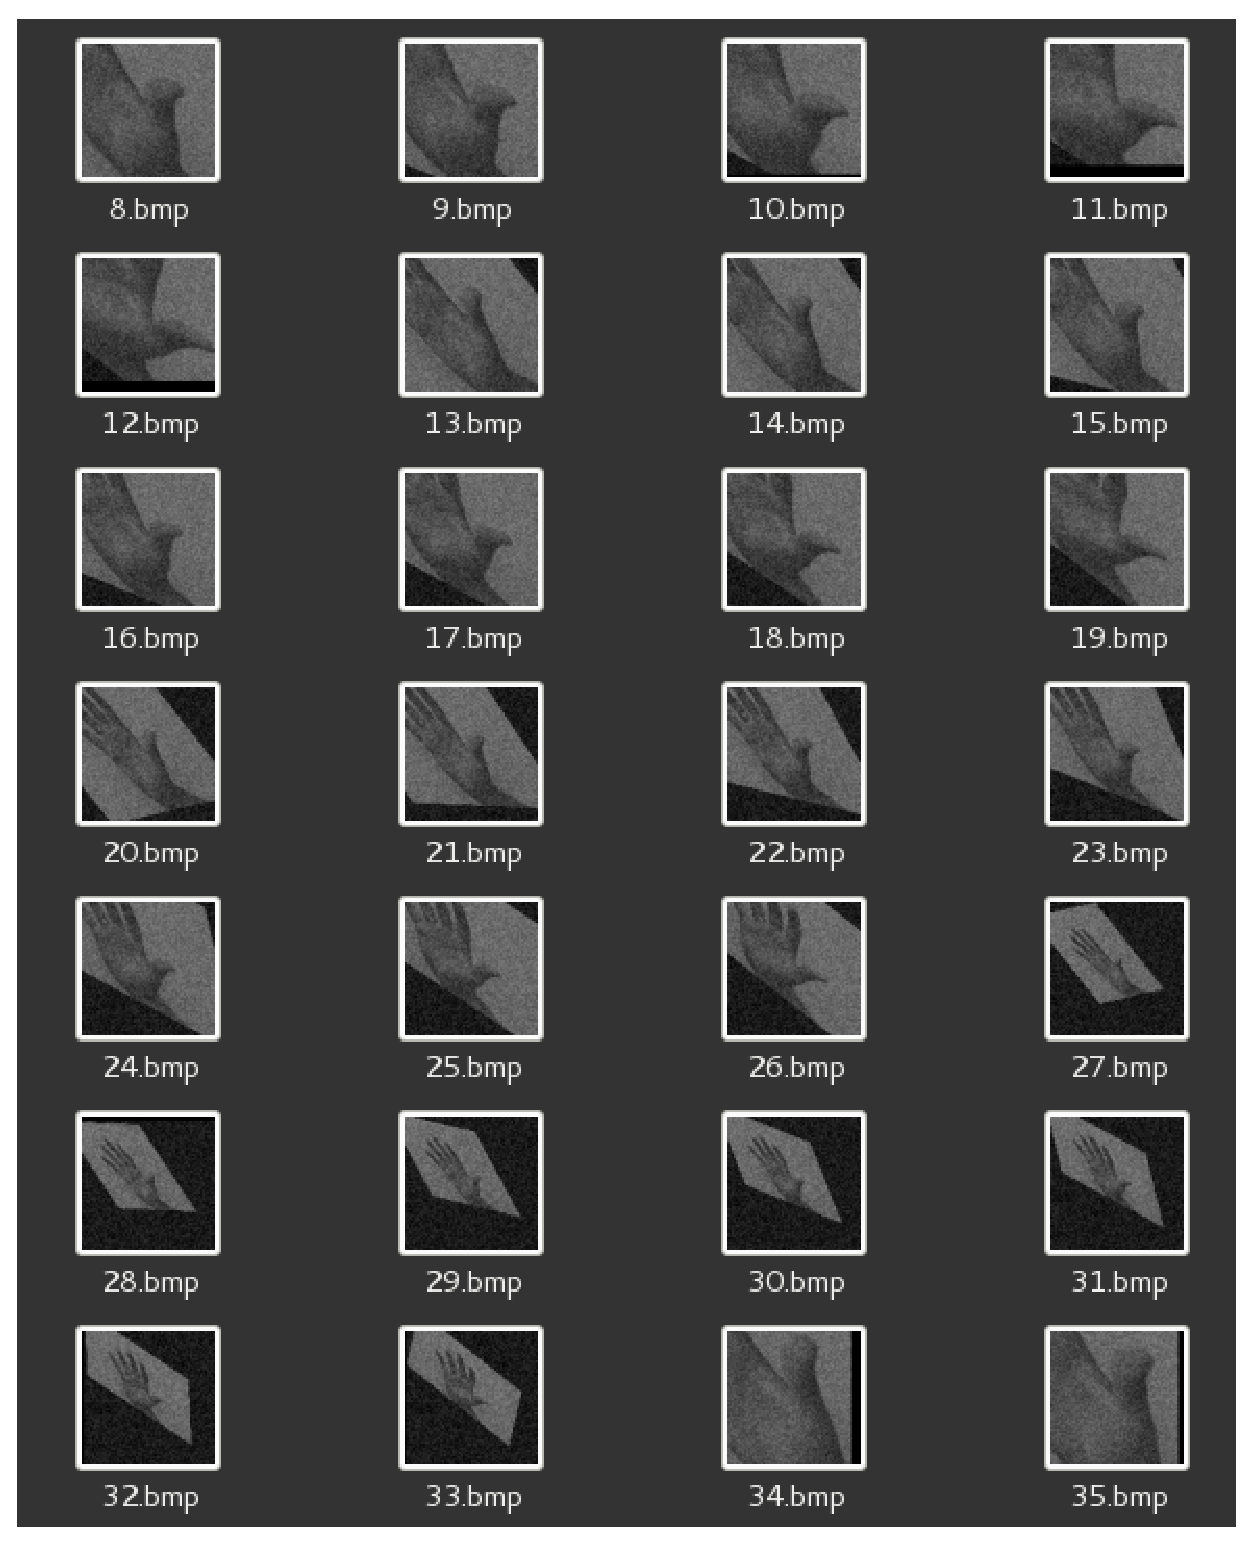
\includegraphics[width=14cm]{GeneratedElements}
    \caption[Fragment wygenerowanych danych treningowych dla sekwencji Person\_A\_Crush]{Fragment wygenerowanych danych treningowych dla sekwencji \\\textit{Person\_A\_Crush}}
    \label{fig:GeneratedElements}
  \end{figure}

  \subsection{Implementacja wewnętrzna lasu drzew losowych}
  Wewnętrzna implementacja lasu drzew losowych opiera się na trzech klasach klasycznych (\textit{RandomForest}, \textit{RandomTreeBuilder}, \textit{RandomForestBuilder}) oraz dwóch szablonach klas (\textit{Tree} oraz \textit{TreeWalker}).

  Głównym elementem jest klasa szablonowa \textit{Tree}, która jest strukturą danych reprezentującą drzewo losowe. Szablon sparametryzowany jest klasą reprezentującą węzeł drzewa oraz maksymalną liczbą dzieci podlegających pod~dany węzeł. Implementacja węzła znajduje się w~klasie \textit{DecisionNode}. Kolejna klasa szablonowa \textit{TreeWalker} enkapsuluje algorytm poruszania się po zbudowanym drzewie (algorytm wykorzystywany jest przy klasyfikacji, zaimplementowanej wewnątrz klasy \textit{RandomForest}).

  Klasa \textit{RandomForest} reprezentuje zbudowaną i~wyuczoną strukturę lasu drzew losowych, dzięki której możliwe jest przeprowadzenie procesu klasyfikacji. Szczegóły algorytmu klasyfikacji zostały omówione w~rozdziale \ref{Subsection_RandomizedTrees}.

  Obiekty omawianej klasy zwracane są jako wynik działania metody \textit{build} klasy \textit{RandomForestBuilder} (wykorzystano wzorzec \textit{budowniczy}, ang. \textit{builder}). Kolejna klasa \textit{RandomTreeBuilder} enkapsuluje algorytm budowy pojedynczego drzewa losowego, wykorzystywany przez wzorzec budowniczego lasu drzew losowych. Tak jak w~poprzednim przypadku tutaj również zastosowanie znalazł wspomniany wzorzec.

  \textit{Budowniczy} (dokładny opis zawarty w~pozycji \cite{PatternsGoF}) jest jednym z~kreacyjnych wzorców projektowych, którego celem jest rozdzielenie sposobu tworzenia obiektów od ich reprezentacji. Innymi słowy, proces tworzenia obiektu podzielony jest na kilka mniejszych etapów a~każdy z~tych etapów może być implementowany na wiele sposobów. Dzięki takiemu rozwiązaniu możliwe jest tworzenie różnych reprezentacji obiektów w~tym samym procesie konstrukcyjnym. Zazwyczaj stosowany jest do konstrukcji obiektów złożonych, których konfiguracja i~inicjalizacja jest procesem wieloetapowym.

  Całą implementację spina klasa \textit{RandomForestTracker} która wykorzystuje omawiane klasy, enkapsuluje logikę budowy, zapisu i~odczytu bazy treningowej oraz obsługuje prezentację rezultatów.

  Warto wspomnieć o~idiomie PIMPL (ang. \textit{pointer to implementation idiom}) wykorzystanym w~celu ukrycia szczegółów implementacji w~klasie reprezentującej algorytm śledzenia wykorzystujący lasy drzew losowych. Omawiany idiom zastosowany został ze względu na skomplikowane szczegóły implementacyjne, która dla użytkowników pliku nagłówkowego są nieistotne i~niepotrzebnie zwiększają złożoność (oraz wpływają negatywnie na czas kompilacji).

  Omawiana klasa jest również implementacją abstrakcji modyfikatora ramki animacji (omówioną w~sekcji \ref{Subsection_VideoStream}), dzięki czemu wyniki klasyfikacji mogą zostać nałożone na wyjściowy strumień wideo oraz rezultaty badań jakościowych i~wydajnościowych udostępnione są do wyższych warstw.

\chapter{Specyfikacja zewnętrzna}\label{Chapter_SpecyfikacjaZewnetrzna}

  \section{Prezentacja i~wizualizacja wyników działania algorytmów}\label{Section_Front}
    Aby ułatwić eksperymentowanie z~dostępnymi parametrami oraz~wykorzystanie algorytmów śledzenia do analizy zebranych sekwencji wideo został stworzony prosty interfejs użytkownika (wykorzystana technologia została szczegółowo umówiona w~rozdziale \ref{Subsection_NodeJS}).

    \begin{figure}[!ht]
      \centering
      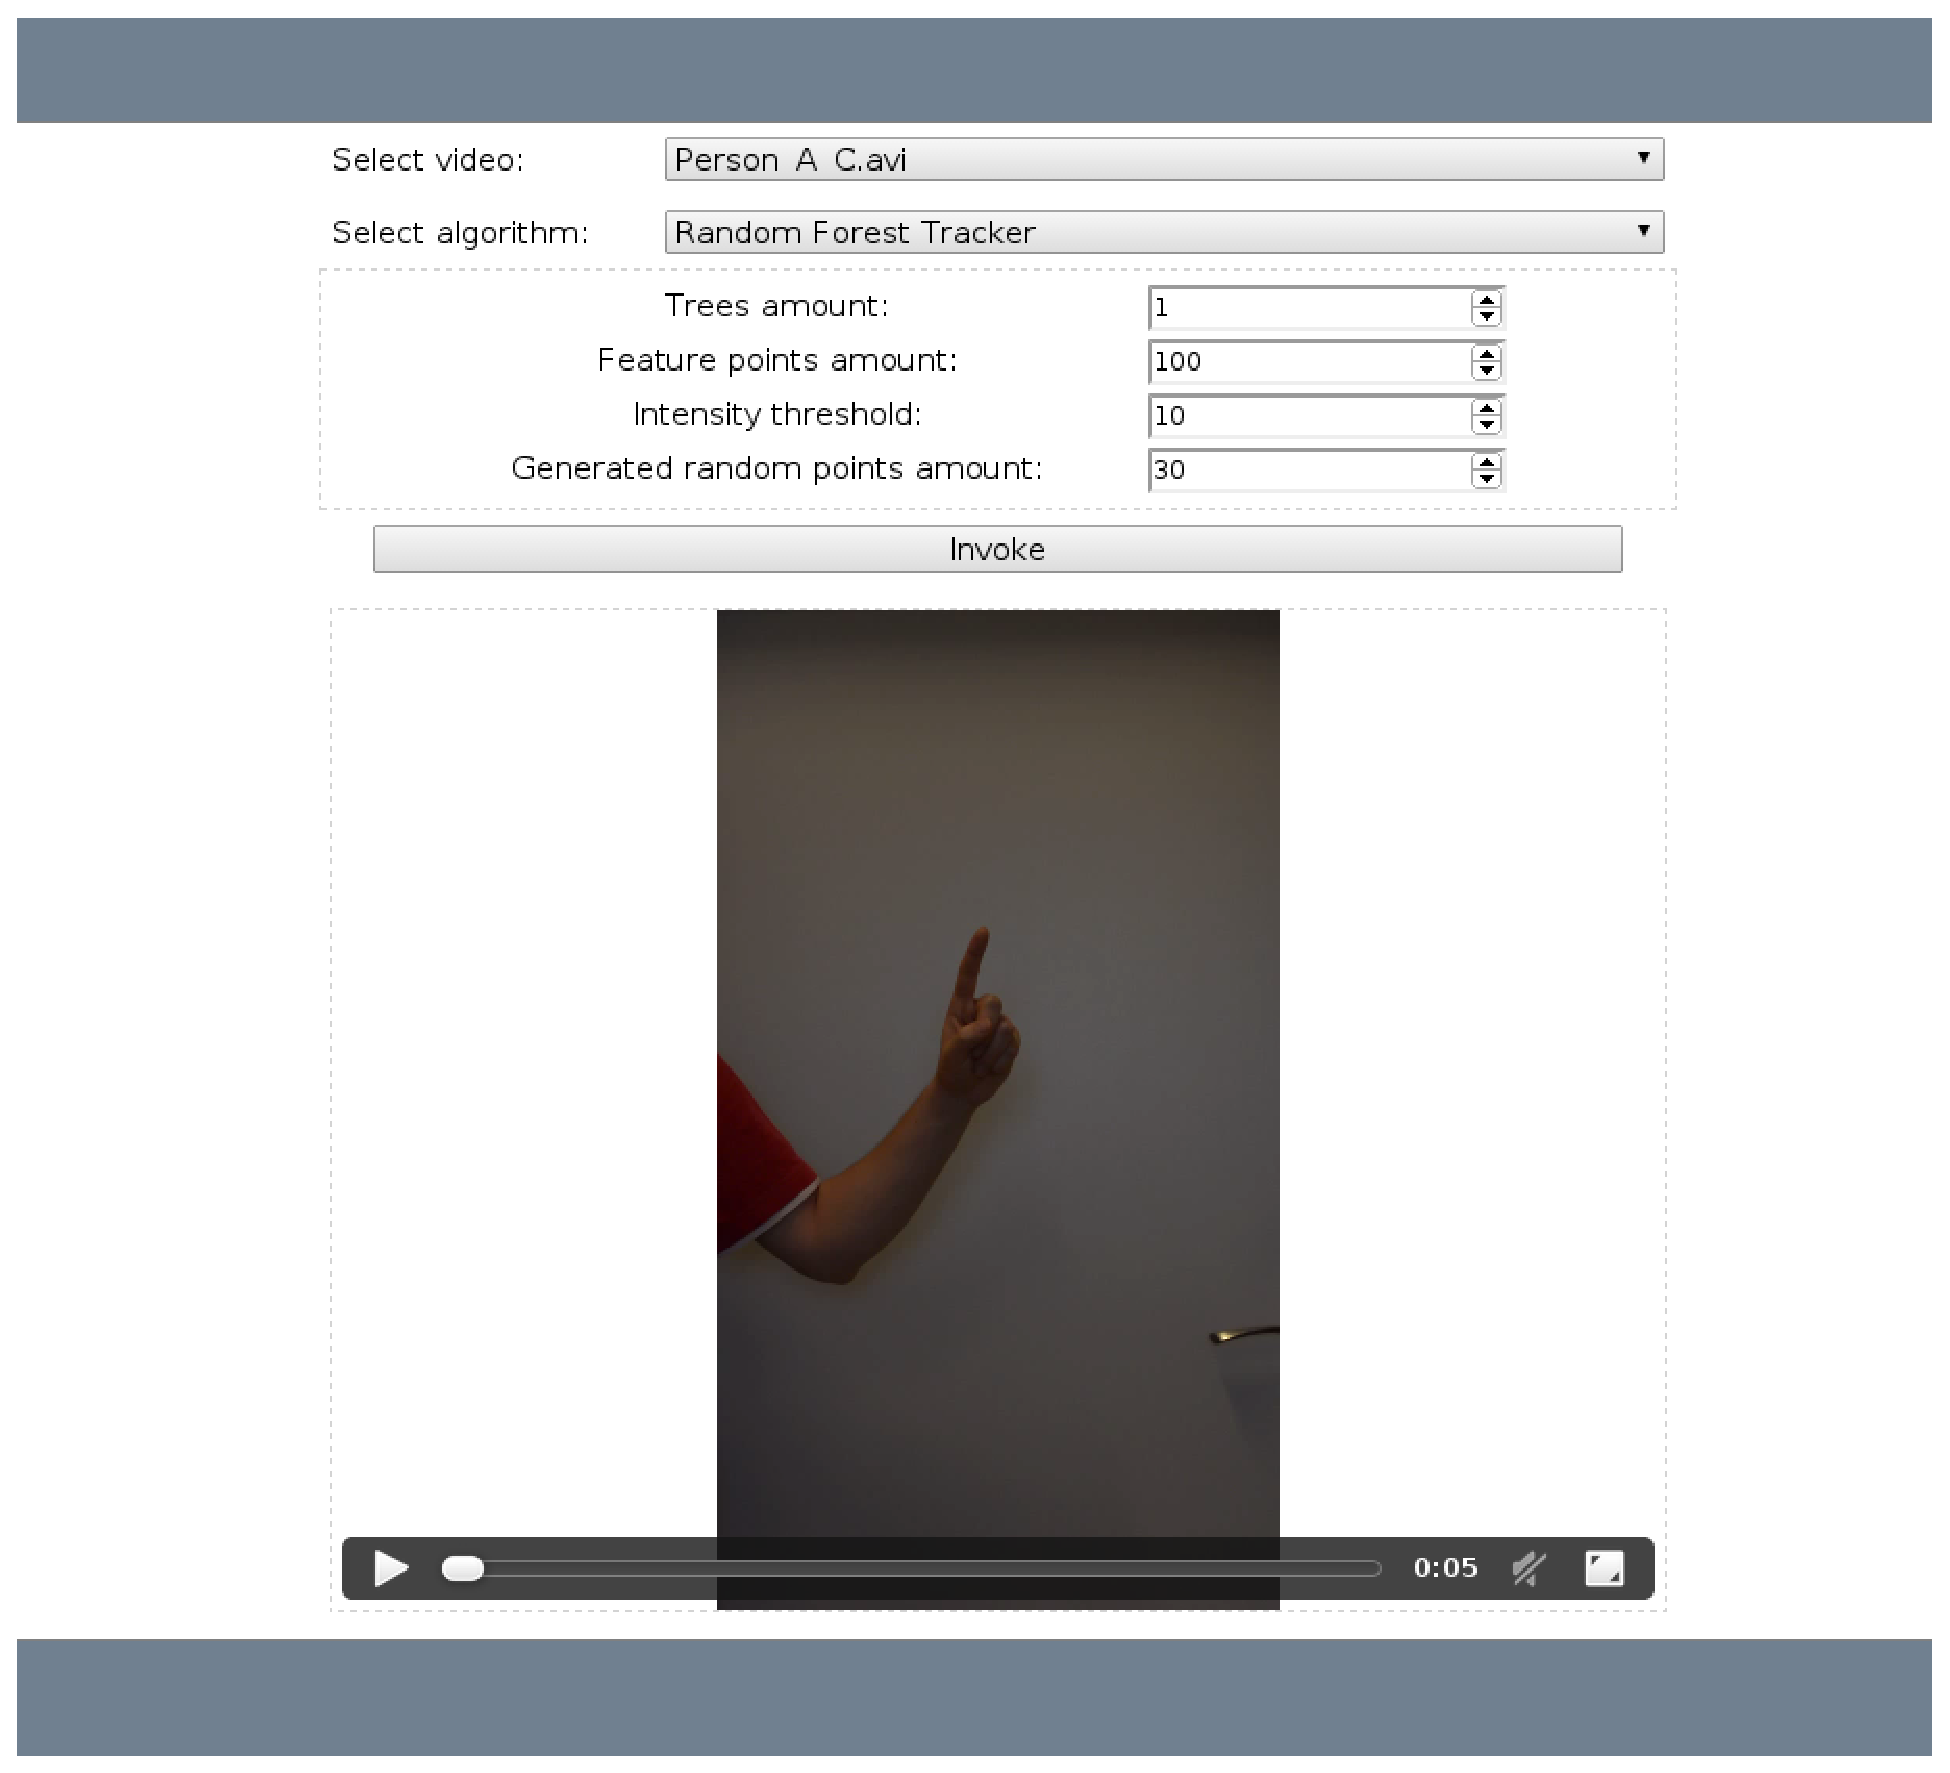
\includegraphics[width=14cm]{Presentation}
      \caption[Interfejs graficzny do prezentacji wyników działania algorytmów]{Interfejs graficzny do prezentacji wyników działania algorytmów}
      \label{fig:AlgorithmsPresentation}
    \end{figure}

    Na rysunku \ref{fig:AlgorithmsPresentation} zaprezentowano jak wygląda stworzony interfejs użytkownika. Z~dwóch pól wyboru zostają podane jako parametry wejściowe nazwa sekwencji wideo oraz nazwa zaimplementowanego algorytmu śledzenia. Poniżej, w~indywidualnym panelu, istnieje możliwość zmiany parametrów dla wybranego sposobu śledzenia punktów charakterystycznych. Istnieje możliwość podglądu wybranej sekwencji za pomocą odtwarzacza wideo.

    Po zaakceptowaniu wyboru, parametry zostają przesłane do serwera pośredniczącego i~po zakończeniu przetworzenia danych odesłana zostanie nowa sekwencja wideo będącą końcowym rezultatem, która może zostać przeglądnięta w~tym samym odtwarzaczu wideo.

  \section{Zaznaczanie punktów kluczowych}\label{Section_Keypoints}
    Każda z~zebranych próbek zgodnie z~protokołem (zamieszczonym w~rozdziale \ref{Section_DefinicjeGestow}) reprezentuje określony kształt lub gest. W~celu wykonania badań jakościowych zaistniała potrzeba zaznaczenia punktów kluczowych połączonych ścieżkami wraz z~otoczeniem samych punktów. Do realizacja zadania został stworzony kolejny interfejs użytkownika.

    \begin{figure}[!ht]
      \centering
      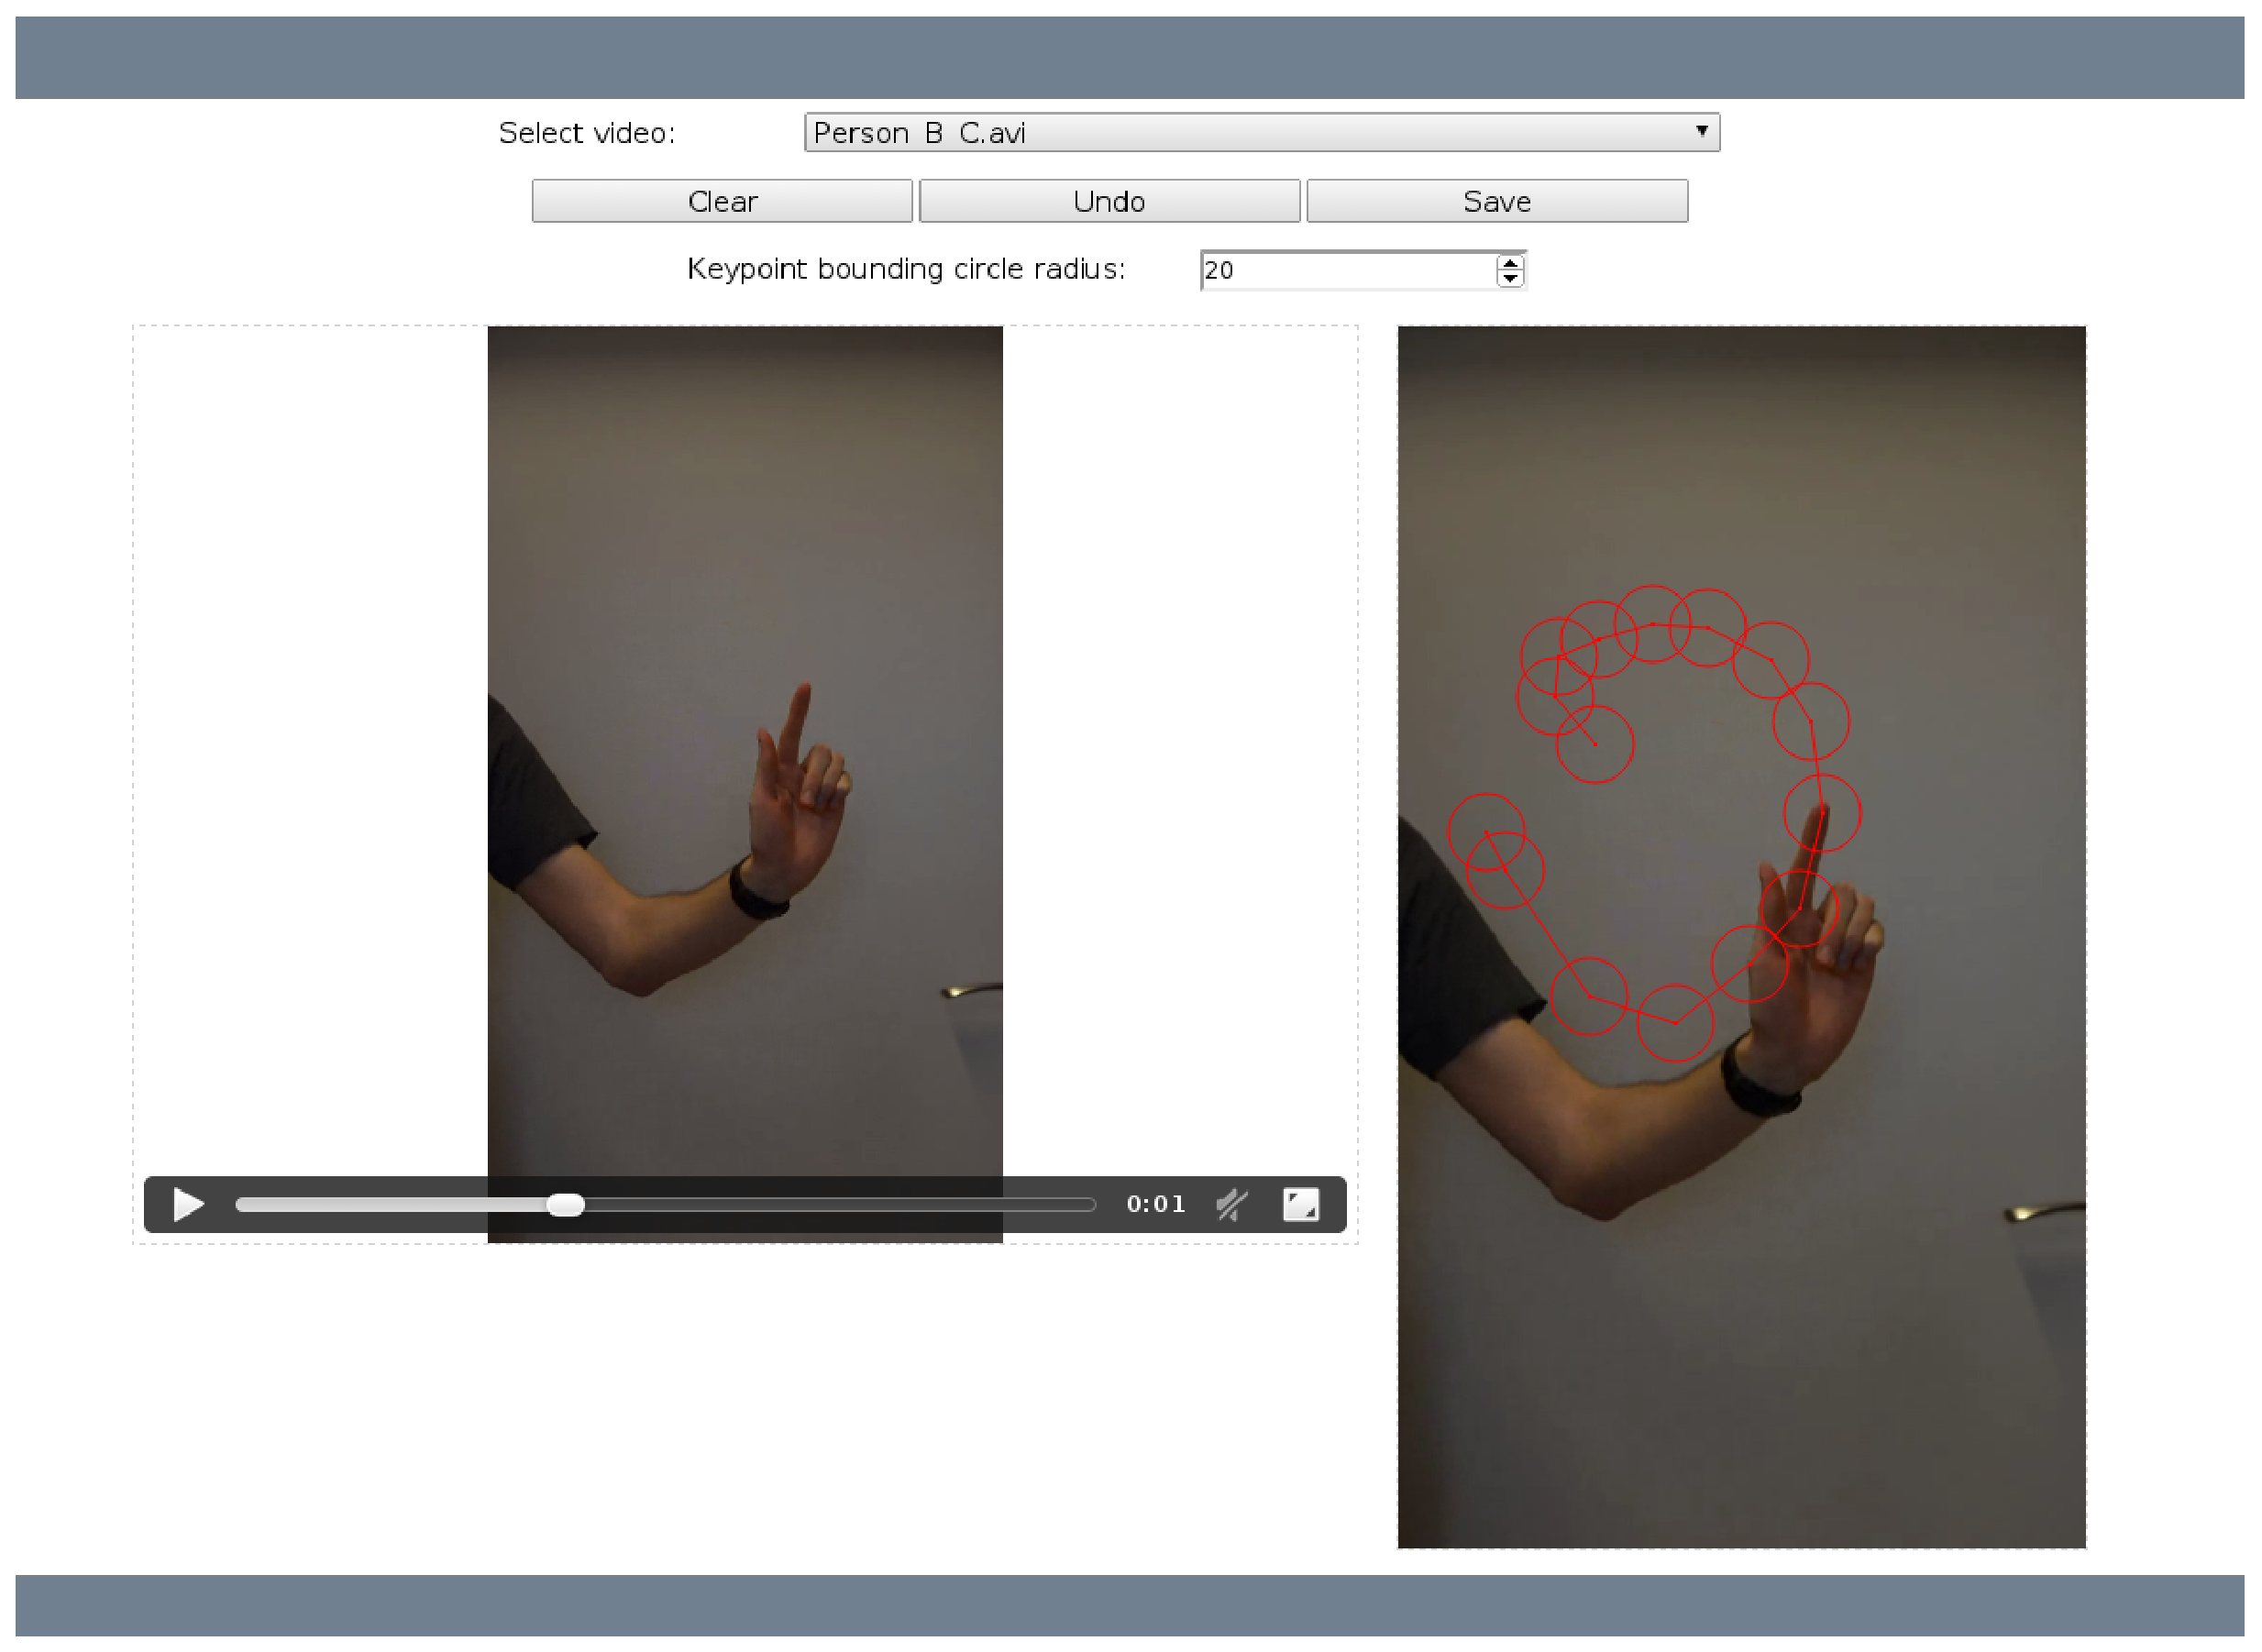
\includegraphics[width=14cm]{Keypoints}
      \caption[Interfejs graficzny do zaznaczania punktów kluczowych]{Interfejs graficzny do zaznaczania punktów kluczowych}
      \label{fig:Keypoints}
    \end{figure}

    Na rysunku \ref{fig:Keypoints} zaprezentowano identyczne pole wyboru sekwencji wideo, odtwarzacz oraz pole robocze do zaznaczania punktów. Po wybraniu odpowiedniej próbki za pomocą odtwarzacza wideo lub strzałek na klawiaturze możliwa jest analiza kolejnych klatek wideo. Na obszarze roboczym za pomocą lewego klawisza myszki zostają zaznaczone kolejne punkty, które zostają kolejno połączone ścieżkami.

    Za pomocą klawiatury (klawisze \textit{U} oraz \textit{R}) lub przycisków istnieje możliwość usunięcia lub przywrócenia ostatnio dodanego punktu. Pole liczbowe służy do manipulacji promieniem okręgów otaczających poszczególne punkty kluczowe.

    Po uzyskaniu najlepszego kształtu, dane mogą zostać wysłane i~zapisane po stronie serwera pośredniczącego do formatu tekstowego (rozszerzenie \textit{keypoints}, format zaprezentowany w~przykładzie \ref{KeypointsTxt}) oraz formatu XML zaprezentowanego w~przykładzie \ref{KeypointsXml}. Pliki z~zapisanymi punktami kluczowymi posiadają taką samą nazwę jak sekwencja wideo.

      \begin{sample}[ht]
        \begin{verbatim}
50
18
364 400
324 394
262 396
228 408
188 452
150 506
126 552
110 596
98 640
110 684
126 728
172 756
220 774
304 794
356 798
400 790
448 768
486 738
        \end{verbatim}
        \caption{Punkty kluczowe w~formacie tekstowym (sekwencja \textit{Person\_A\_C})}
        \label{KeypointsTxt}
      \end{sample}

    \newpage
      \begin{sample}[ht]
        \begin{verbatim}
<?xml version="1.0" encoding="utf-8"?>
<FeaturePointList>
    <hand>
        <FeaturePointRadius r="50" />
        <FeaturePoint x="364" y="400" />
        <FeaturePoint x="324" y="394" />
        <FeaturePoint x="262" y="396" />
        <FeaturePoint x="228" y="408" />
        <FeaturePoint x="188" y="452" />
        <FeaturePoint x="150" y="506" />
        <FeaturePoint x="126" y="552" />
        <FeaturePoint x="110" y="596" />
        <FeaturePoint x="98" y="640" />
        <FeaturePoint x="110" y="684" />
        <FeaturePoint x="126" y="728" />
        <FeaturePoint x="172" y="756" />
        <FeaturePoint x="220" y="774" />
        <FeaturePoint x="304" y="794" />
        <FeaturePoint x="356" y="798" />
        <FeaturePoint x="400" y="790" />
        <FeaturePoint x="448" y="768" />
        <FeaturePoint x="486" y="738" />
    </hand>
</FeaturePointList>
        \end{verbatim}
        \caption{Punkty kluczowe w~formacie XML (sekwencja \textit{Person\_A\_C})}
        \label{KeypointsXml}
      \end{sample}

  \section{Interfejs linii komend programu przetwarzającego sekwencje wideo}\label{Section_CLI}
    Omawiany program jest sercem implementacyjnym całej pracy. Do niego serwer pośredniczący przesyła parametry wejściowe i~po zakończeniu jego działania wysyła rezultaty z~powrotem do interfejsu graficznego. Również rezultaty badań jakościowych oraz wydajnościowych są prezentowane za jego pomocą (jak widać na obrazie \ref{fig:Cli} służy do tego opcjonalny przełącznik \textit{-{}-include-results}).

    \newpage
    \begin{figure}[!ht]
      \centering
      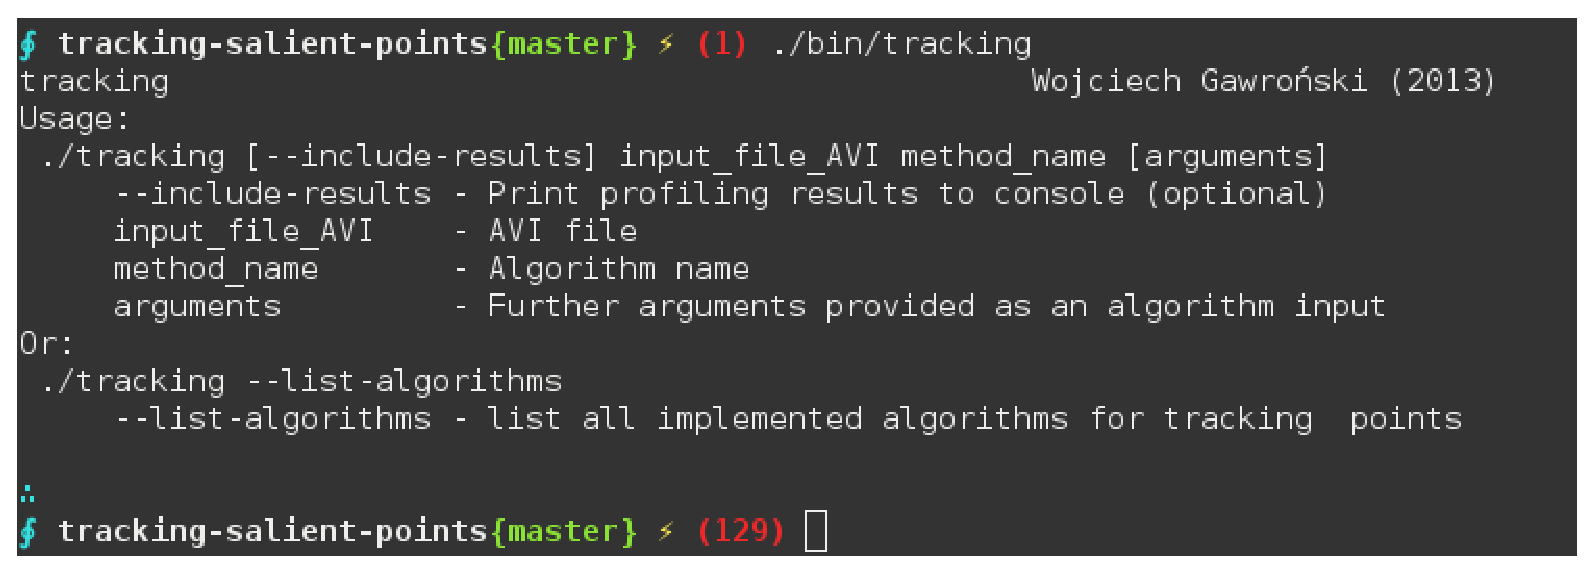
\includegraphics[width=14cm]{Cli}
      \caption[Interfejs linii komend programu do przetwarzania sekwencji wideo]{Interfejs linii komend programu do przetwarzania sekwencji wideo}
      \label{fig:Cli}
    \end{figure}

    Poniżej, w~listingu \ref{SampleInvoke}, został zamieszczony przykład wywołania (wywołanie wykonane z~głównego katalogu źródłowego):

    \begin{sample}[ht]
      \begin{verbatim}
./bin/tracking assets/Person_A_C.avi "Random Forest Tracker" 30 100
      \end{verbatim}
      \caption{Przykładowe wywołanie interfejsu konsolowego}
      \label{SampleInvoke}
    \end{sample}

    Program dostarcza również listy zaimplementowanych algorytmów (prezentowanej w~interfejsie użytkownika, w~polu wyboru algorytmu śledzenia) uzyskiwanej za pomocą przełącznika \textit{-{}-list-algorithms}.

    Wywołanie interfejsu linii komend bez parametrów (lub z~niewystarczającą liczbą argumentów) pokaże instrukcję użycia, widoczną również na rysunku \ref{fig:Cli}.

  \section{Interfejs użytkownika do prezentacji wykresów i~wyników badań}

    Zupełnie odrębnym widokiem zaprojektowanym i~zaimplementowanym w~aplikacji jest prezentacja wykresów z~zebranych danych pomiarowych. Widok został zbudowany w~oparciu o~technologie szczegółowo omówione w~rozdziale \ref{Subsection_PomocniczeTechnologie}. Na rysunku \ref{fig:Charts} został zaprezentowany przykładowy wykres.

    \newpage
    \begin{figure}[!ht]
      \centering
      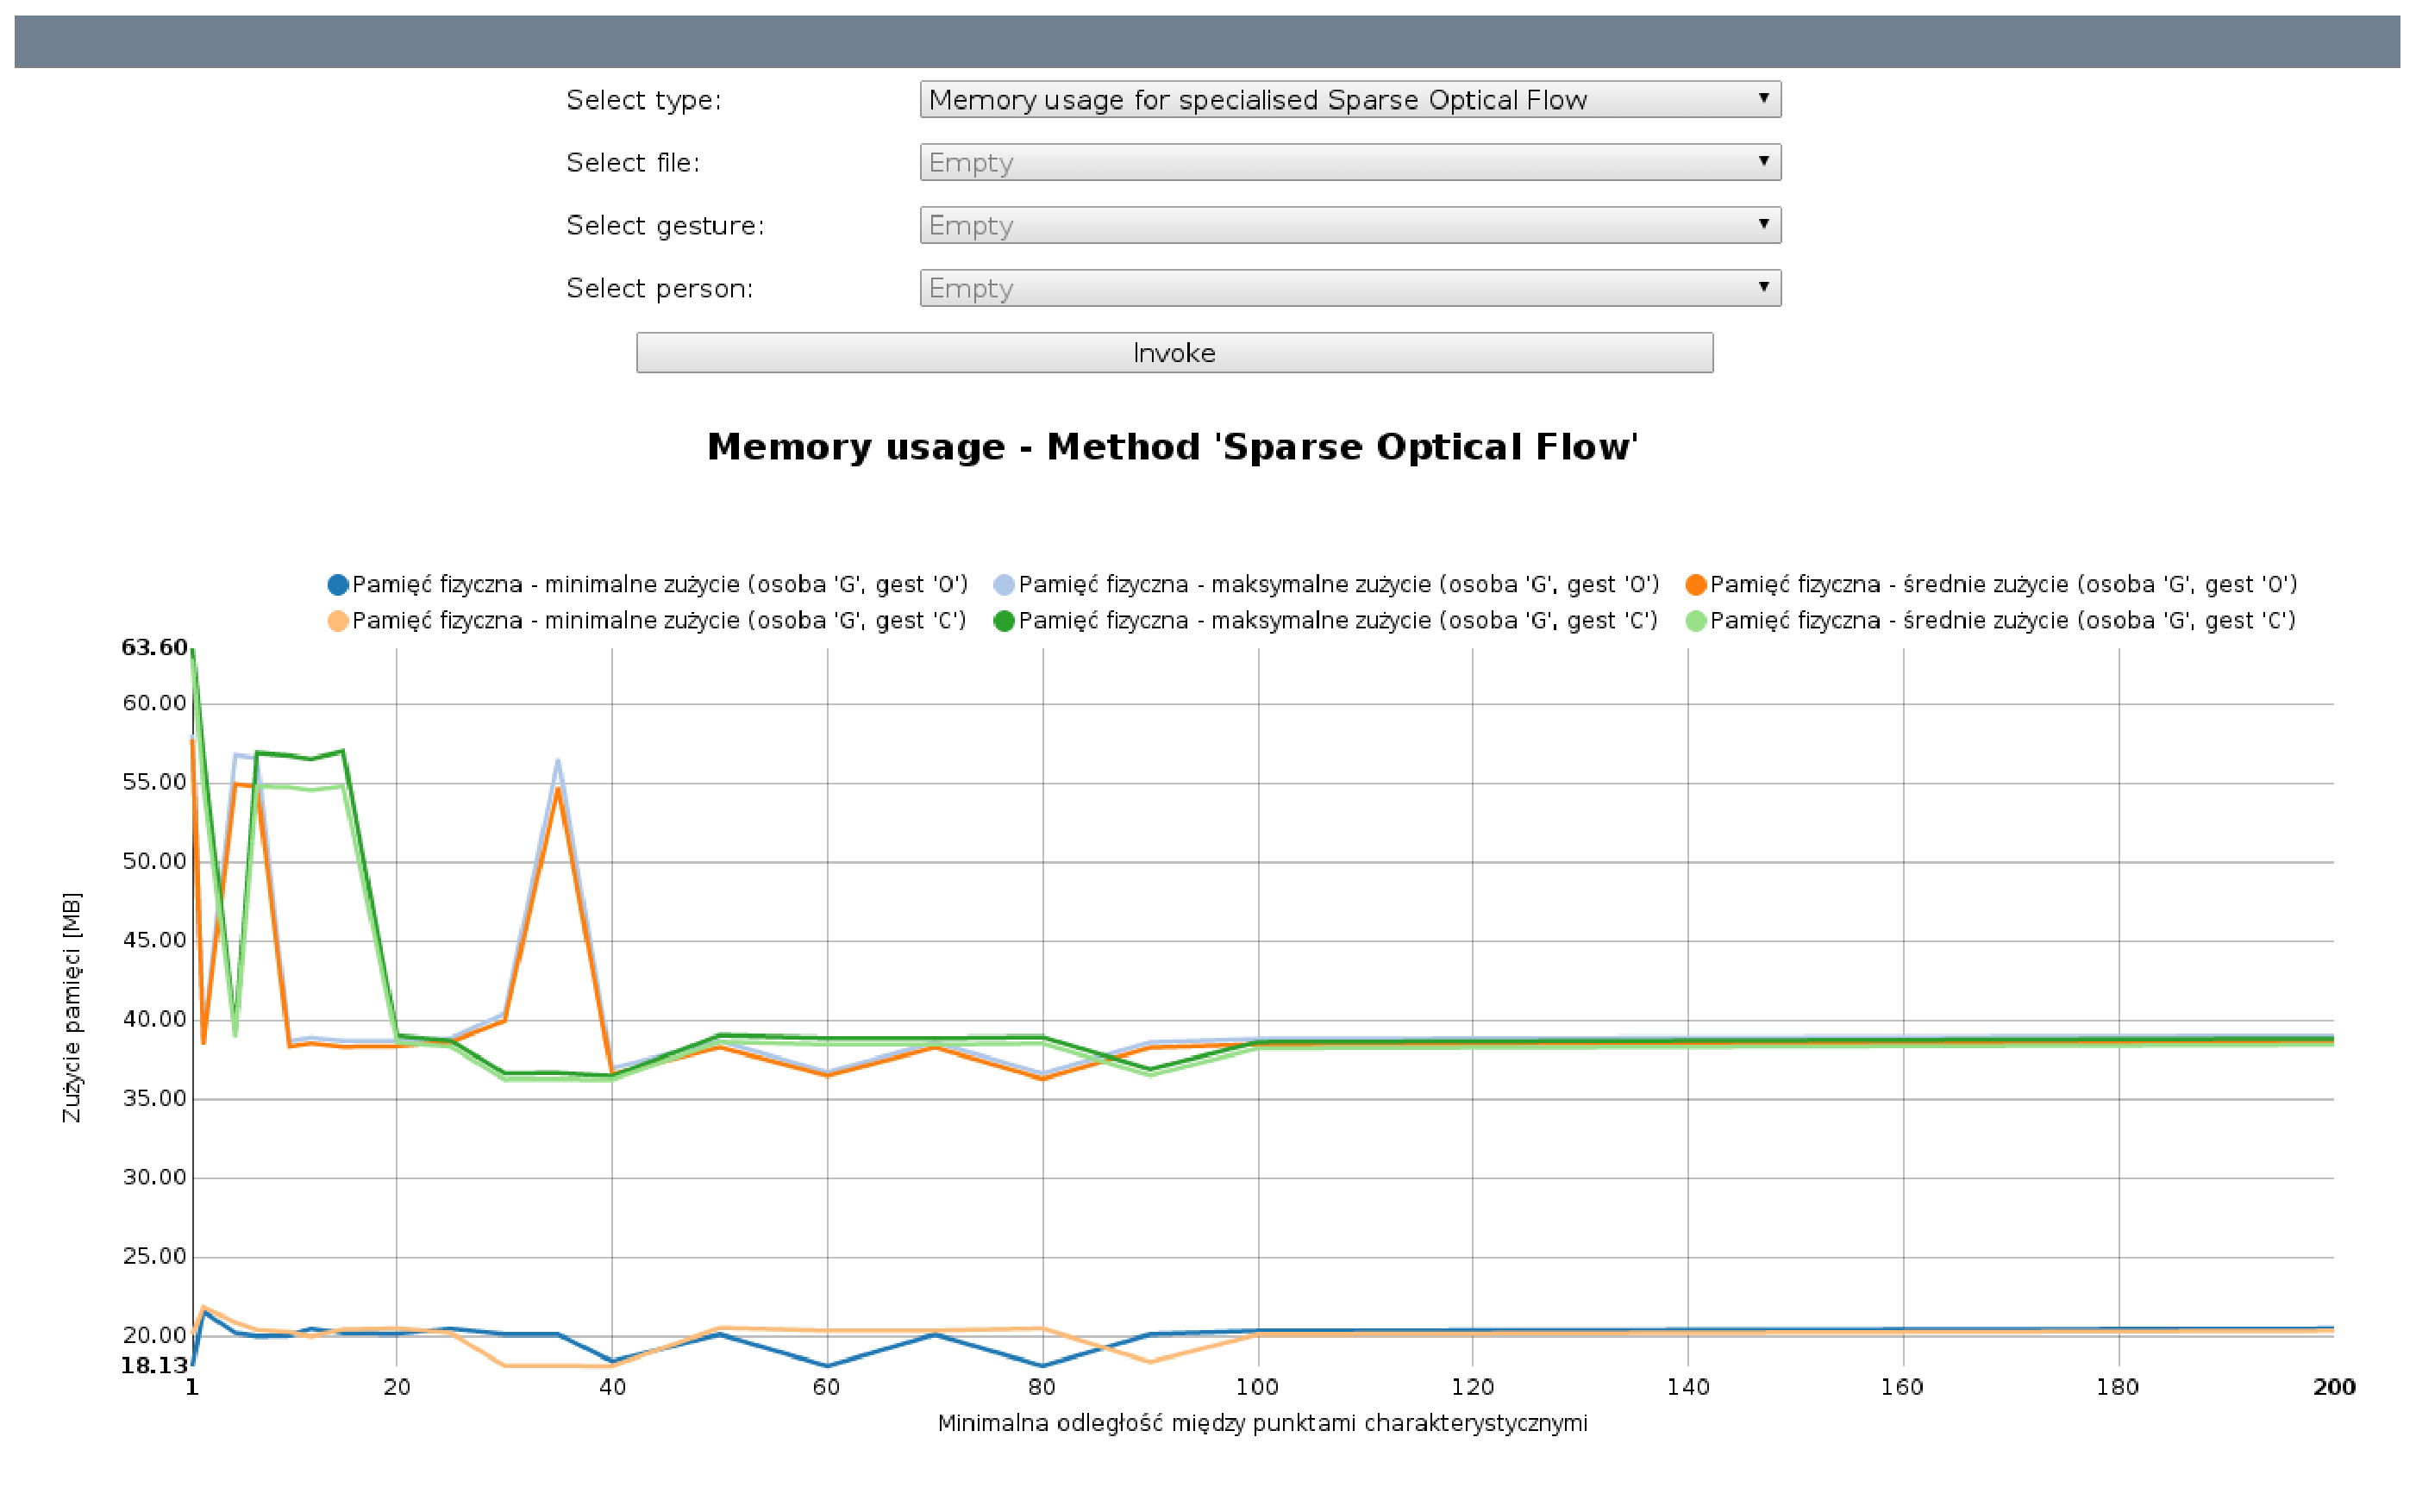
\includegraphics[width=14cm]{Charts}
      \caption[Interfejs graficzny służący do prezentacji wykresów]{Interfejs graficzny służący do prezentacji wykresów}
      \label{fig:Charts}
    \end{figure}

    Użytkownik za pomocą pól wyboru umieszczonych w~górnej części interfejsu ma możliwość wybrania typu wykresu oraz ustawienia odpowiednich parametrów. Po zaznaczeniu określonych opcji (oraz krótkiej chwili, ponieważ generacja oraz rysowanie wykresu jest procesem kosztownym obliczeniowo) w~oknie przeglądarki pojawią się wygenerowane rezultaty.

    Prezentacja wybranych wykresów na jednej stronie ułatwia porównywanie poszczególnych wyników. Stworzone wykresy są interaktywne - możliwe jest wyłączenie poszczególnych serii oraz sprawdzenie dokładnej wartości jaka znajduje się w~danym punkcie.

    Warto nadmienić, że rezultaty zamieszczone w~pracy w~rozdziale \ref{Chapter_AnalizaRezultatow} zostały stworzone za pomocą tego widoku.